\begin{figure}[htp]
  \centering
  \subfloat[Ranking based on a high convex hull percentage]{\label{figur:1}
\includegraphics[width=0.45\textwidth]{figures/convexitypercentage.png}}
  \hfill
  \subfloat[Ranking based on a low number of outline vertices]{\label{figur:2}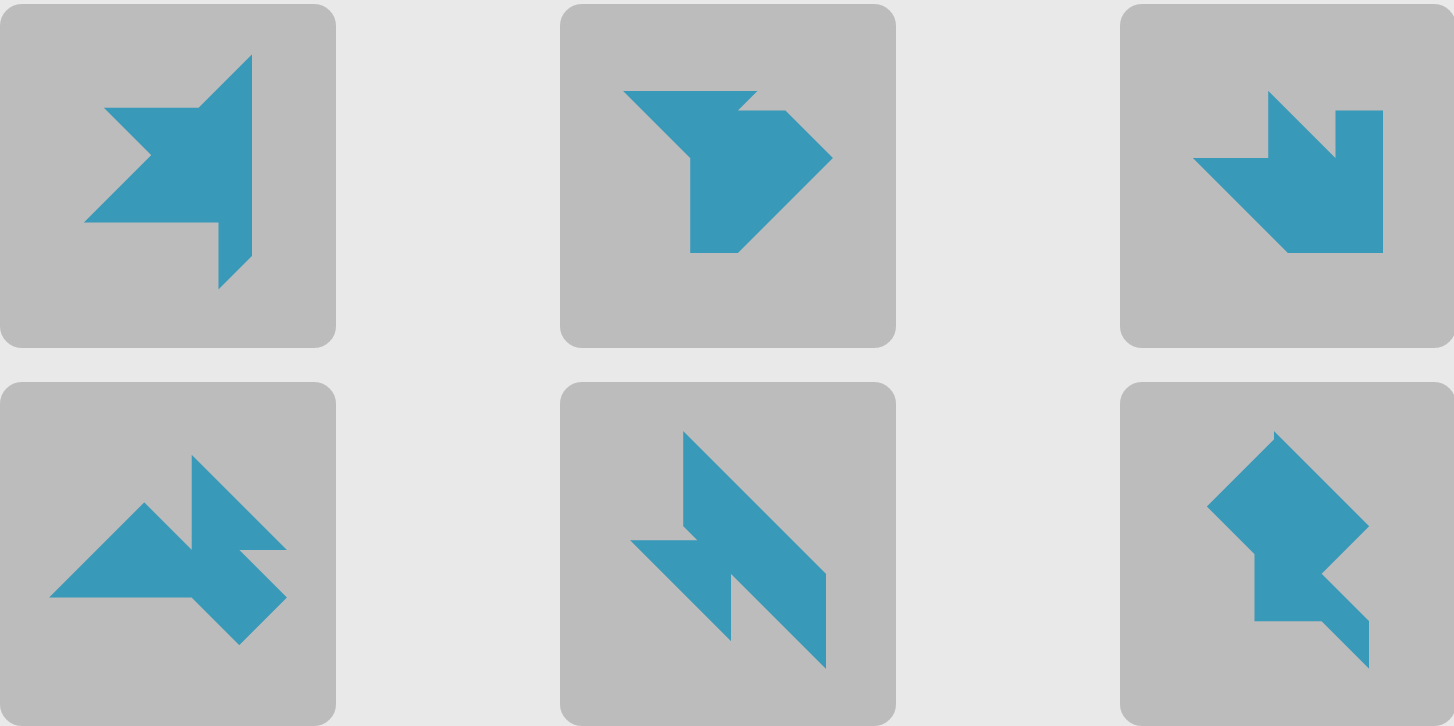
\includegraphics[width=0.45\textwidth]{figures/outlineVertices.png}}
  \\
  \subfloat[Ranking based on a high convex hull percentage and a low number of outer outline vertices]{\label{figur:4}
\includegraphics[width=0.45\textwidth]{figures/combineOuter.png}}
    \hfill
  \subfloat[Ranking based on a high number of matched vertices]{\label{figur:5}
\includegraphics[width=0.45\textwidth]{figures/matchedV.png}}
\caption{Results of generating 10.000 tangrams and ranking them according to different interestingness measures}
\label{eval2}
\end{figure}